\chapter{Differential Equations}
\thispagestyle{fancy}
\begin{defn}[Del Operator]{1}
	The Del operator with respect to $n$-dimensions:
\begin{align}
\nabla &= \bigg( \frac{\partial}{\partial x_1}, \frac{\partial}{\partial x_2}, \dots, \frac{\partial}{\partial x_n} \bigg) = \sum_{i=1}^{n}\vec{e}_i\frac{\partial}{\partial x_i}
\end{align}
\end{defn}
The \textbf{gradient}\index{Gradient} of a 3-dimensional function (cartesian, spherical, and cylindrical coordinates)
\begin{align}
\textrm{grad } f = \nabla f &= \frac{\partial f}{\partial x}\hat{x}+\frac{\partial f}{\partial y}\hat{y}+\frac{\partial f}{\partial z}\hat{z} \\
&=\frac{\partial f}{\partial r}\hat{r}+\frac{1}{r}\frac{\partial f}{\partial \theta}\hat{\theta}+\frac{1}{r\sin(\theta)}\frac{\partial f}{\partial \phi}\hat{\phi} \\
&=\frac{\partial f}{\partial \rho}\hat{\rho}+\frac{1}{\rho}\frac{\partial f}{\partial \phi}\hat{\phi}+\frac{\partial f}{\partial z}\hat{z}
\end{align}
The \textbf{curl}\index{Curl} of a vector is the limit as the volume goes to zero of the ratio of the integral of it's cross product (with respect to the normal) over a closed surface, to the volume enclosed by the surface \cite{bib:ReitzEMTheory}. The curl of a 3-dimensional function (cartesian, spherical, and cylindrical coordinates)
\begin{align}
\textrm{curl } \vec{A} = \nabla \times \vec{A} &= \lim\limits_{V\rightarrow 0}\frac{1}{V}\oint_S(\hat{n}\times \vec{A})da\hspace{2cm}\textrm{(definition)} \\
&= \bigg( \frac{\partial A_z}{\partial y} -\frac{\partial A_y}{\partial z}\bigg)\hat{x}+\bigg( \frac{\partial A_x}{\partial z} -\frac{\partial A_z}{\partial x}\bigg)\hat{y}+\bigg( \frac{\partial A_y}{\partial x} -\frac{\partial A_x}{\partial y}\bigg)\hat{z} \\ &= \frac{1}{r\sin(\theta)}\bigg[\frac{\partial}{\partial \theta}\sin(\theta)A_\phi-\frac{\partial A_\theta}{\partial \phi}\bigg]\hat{r}+\bigg[\frac{1}{r\sin(\theta)}\frac{\partial A_r}{\partial \phi}-\frac{1}{r}\frac{\partial}{\partial r}(rA_\phi) \bigg]\hat{\theta} \nonumber \\
& \hspace{6cm}+ \frac{1}{r}\bigg[\frac{\partial}{\partial r}(rA_\theta)-\frac{\partial A_r}{\partial \theta} \bigg]\hat{\phi} \\
&= \bigg[\frac{1}{\rho}\frac{\partial A_z}{\partial \phi}-\frac{\partial A_\phi}{\partial z} \bigg] \hat{\rho} + \bigg[\frac{\partial A_\rho}{\partial z}-\frac{\partial A_z}{\partial \rho}  \bigg]\hat{\phi} + \frac{1}{\rho}\bigg[\frac{\partial}{\partial \rho}(\rho A_\phi)-\frac{\partial A_\rho}{\partial \phi} \bigg]\hat{z} 
\end{align}
The \textbf{divergence}\index{Divergence} of a vector is the limit of its surface integral per unit volume as the volume enclosed by the surface goes to zero \cite{bib:ReitzEMTheory}. The divergence of a 3-dimensional function (cartesian, spherical, and cylindrical coordinates) is
\begin{align}
\textrm{div }\vec{A}=\nabla \cdot \vec{A} &= \lim\limits_{V\rightarrow 0}\frac{1}{V}\oint_S (\vec{A}\cdot \hat{n}) da \hspace{2cm}\textrm{(definition)} \\ &=\frac{\partial A_x}{\partial x} + \frac{\partial A_y}{\partial y} + \frac{\partial A_z}{\partial z} \\
&= \frac{1}{r^2}\frac{\partial}{\partial r}(r^2A_r)+\frac{1}{r\sin(\theta)}\frac{\partial}{\partial \theta}\sin(\theta)A_\theta+\frac{1}{r\sin(\theta)} \frac{\partial A_\phi}{\partial \phi} \\
&= \frac{1}{\rho}\frac{\partial}{\partial \rho}(\rho A_\rho) + \frac{1}{\rho}\frac{\partial A_\phi}{\partial \phi}+ \frac{\partial A_z}{\partial z}
\end{align}
The Laplace Operator (expanded in 3-dimensions below)
\begin{align}
\Delta = \nabla \cdot \nabla = \nabla^2 =  \frac{\partial^2}{\partial x^2}+ \frac{\partial^2}{\partial y^2}+ \frac{\partial^2}{\partial z^2}
\end{align}
The general solution to Laplaces equation in spherical coordinates with no $\phi$ dependence (where $P_\ell$ denotes the Legendre polynomials) is
\begin{align}
	\nabla^2 V(r,\theta) = 0 \implies V(r,\theta) = \sum_{\ell=0}^{\infty}\left(A_\ell r^\ell+\frac{B_\ell}{r^{\ell+1}}\right)P_\ell(\cos\theta)
\end{align}



\section{Differentiation}
\begin{defn}[Derivative of a function]{1}
	The derivative of a function represents an infinitesimal change in the function with respect to one of its variables. Let $f:\mathbb{R}\rightarrow\mathbb{R}$. Then the derivative of $f$ with respect to a variable $x$ is given by
	\begin{align}
	\frac{d}{dx}f(x)\equiv f'(x) \equiv\lim\limits_{\Delta x \rightarrow 0}\frac{f(x+\Delta x)-f(x)}{\Delta x} \equiv \lim\limits_{\Delta x \rightarrow 0}\frac{f(x+\Delta x)-f(x-\Delta x)}{2\Delta x}
	\end{align}
\end{defn} 
\begin{defn}[Partial Derivative of a function]{1}
	Partial derivatives are defined as derivatives of a function of multiple variables when all but the variable of interest are held fixed during the differentiation. Let $f:\mathbb{R}^z\rightarrow\mathbb{R}$, with $z \in \mathbb{N}$. Then the partial derivative of $f$ with respect to a variable $x_m$ is given by
	\begin{align}
	\frac{\partial}{\partial x_m}f(x_1,\dots,x_n) \equiv \lim\limits_{\Delta x \rightarrow 0}\frac{f(x_1,\dots,x_m+\Delta x, \dots,x_n)-f(x_1,\dots,x_m,\dots,x_n)}{\Delta x}
	\end{align}
\end{defn}
\begin{fancybox}[Derivative of an $n^{th}$ degree polynomial.]{}
	Let $f:\mathbb{R}\rightarrow\mathbb{R}$ such that $f(x)\in\mathbb{P}_n$ of the form $f(x)=b_nx^n+b_{n-1}x^{n-1}+\cdots++b_1x+b_0$. Then the $m^{\textrm{th}}$ derivative of $f(x)$ is given by
	\begin{align}
	\frac{d^m}{dx^m}f(x)=f^{(m)}(x)=\sum_{k=0}^{n-m}\frac{(n-k)!}{(n-m-k)!}b_{n-k}x^{n-m-k}.
	\end{align}
\end{fancybox}
\begin{fancybox}[Derivative of a sum of simple exponential functions]{}
	Let $f:\mathbb{R}\rightarrow\mathbb{R}$ be a continuous function such that $f(x)=b_n e^{k_n x}+b_{n-a}e^{k_{n-1}x}+\cdots+b_1e^{k_1x}+b_0e^{k_0x}$, with $b_n$ and $k_n$ as constants. The $m^\textrm{th}$ derivative is then given by
	\begin{align}
	\frac{d^m}{dx^m}f(x)=\frac{d^m}{dx^m}\sum_{i=0}^{n}b_ie^{k_ix}=\sum_{i=0}^{n}b_{n-i} k_{n-i}^m e^{k_{n-i} x}.
	\end{align}
\end{fancybox}

\invisiblesection{Review of Differentiation}
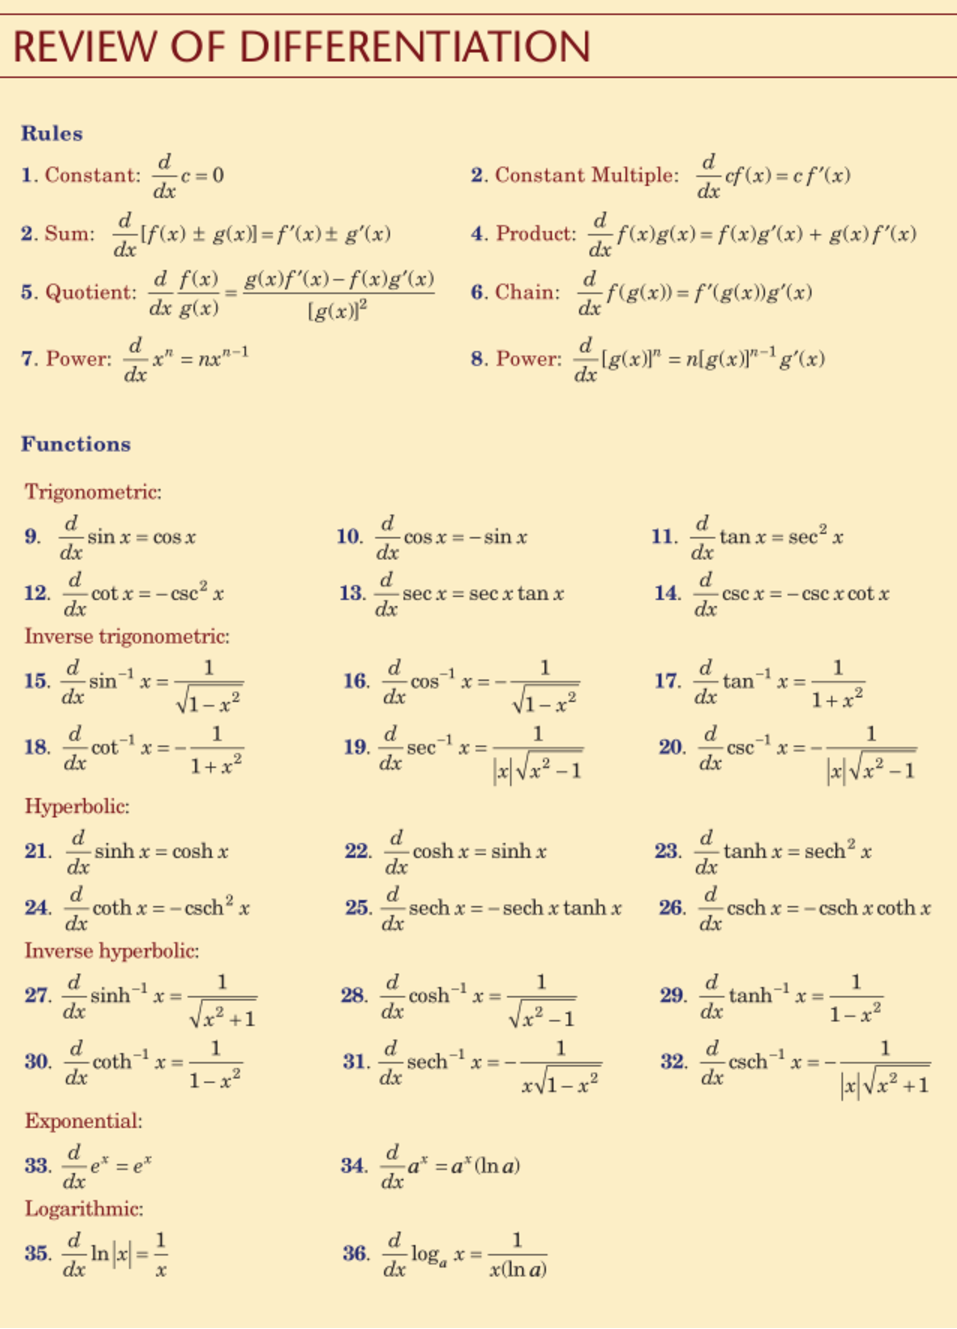
\includepdf[pages=1,pagecommand=\thispagestyle{fancy}, scale=0.8, pagecommand={\footnotetext{This "Review of Differentiation" is taken directly from Dennis G. Zill - A First Course in Differential Equations, 10th Ed. When time permits it will be re-created in an original format.}}]{Resources/DiffEQTable}
\newpage
\begin{fancybox}[Repeating product rule applied to arbitrary functions]{}
	Let $f:\mathbb{R}\rightarrow\mathbb{R}$ and $g:\mathbb{R}\rightarrow\mathbb{R}$ be continuous and differentiable functions of the variable $x$. Then the $m^{\textrm{th}}$ derivative of $f(x)g(x)$ with respect to $x$ is
	\begin{align*}
	\frac{d^m}{dx^m}f(x)g(x)=\sum_{i=0}^{n}{{n}\choose{i}}\bigg[\frac{d^i}{dx^i}f(x) \bigg]\bigg[\frac{d^{n-i}}{dx^{n-i}}g(x) \bigg].
	\end{align*}
\end{fancybox}




\section{Legendre differential equation}
The \textbf{Legendre polynomials}\index{Legendre polynomials} are normalized solutions to the Legendre differential equation
\begin{align}
	(1-x^2)\frac{d^2y}{dx^2}-2x\frac{dy}{dx}+\ell(\ell+1)y=0.
\end{align}
which have the general solution below. For even $\ell$, we must take $a_1 = 0$ to obtain a convergent solution, and for odd $\ell$, we must take $a_0 = 0$.
\begin{align}
	y=&a_0\left[1-\frac{\ell(\ell+1)}{2!}x^2+\frac{\ell(\ell+1)(\ell-2)(\ell+3)}{4!}x^4-\cdots\right] \\&+a_1\left[x-\frac{(\ell-1)(\ell+2)}{3!}x^3+\frac{(\ell-1)(\ell+2)(\ell-3)(\ell+4)}{5!}x^5-\cdots\right]
\end{align}
The Legendre polynomial $P_\ell(z)$ can be defined by the contour integral
\begin{align}
	P_\ell(z) = \frac{1}{2\pi i}\oint (1-2tz+t^2)^{-1/2}t^{-\ell-1} dt.
\end{align}
The first few Legendre Polynomials follow as:
\begin{multicols}{2}
	\noindent
\begin{align}
	P_0(x) &=1 \\
	P_1(x) &= x \\
	P_2(x) &= \frac{1}{2}(3x^2-1) \\
	P_3(x) &= \frac{1}{2}(5x^3 -3x) 
\end{align}
\begin{align}
	P_4(x) &= \frac{1}{8}(35x^4 - 30x^2 +3) \\
	P_5(x) &= \frac{1}{8}(63x^5-70x^3+15x) \\
	&\vdots \nonumber
\end{align}
\end{multicols}
The Rodrigues representation provides a formula for solving for the Legendre Polynomials
\begin{align}
	P_\ell(x) = \frac{1}{2^\ell \ell!}\frac{d^\ell}{dx^\ell}(x^2-1)^\ell
\end{align}
The Legendre polynomials are orthogonal over $(-1,1)$ with weighting function 1 and satisfy
\begin{align}
	\int_{-1}^{1}P_m(x)P_n(x)dx = \frac{2}{2n+1}\delta_{mn} \hspace{1cm} \textrm{and}\hspace{1cm}	\int_{0}^{1}P_m(x)P_n(x)dx = \frac{1}{2n+1}\delta_{mn}
\end{align} 
The associated Legendre differential equation is given by
\begin{align}
	\frac{d}{dx}\left[(1-x^2)\frac{dy}{dx}\right]
	+\left[\ell(\ell-1)-\frac{m^2}{1-x^2}\right]y=0
\end{align}
When $m,\ell \in \mathbb{Z}^+$ and $m \leq \ell$, the solutions to the above  equation are the \textbf{associated Legendre polynomials},
\begin{align}
	P_\ell^m(x) = (-1)^m(1-x^2)^{m/2}\frac{d^m}{dx^m}P_\ell(x) = \frac{(-1)^m}{2^\ell \ell!}(1-x^2)^{m/2}	\frac{d^{\ell+m}}{dx^{\ell+m}}(x^2-1)^\ell
\end{align}
The associated Legendre polynomials for $m < 0$ are defined by
\begin{align}
	P_\ell^{-m}(x) = (-1)^m \frac{(\ell - m)!}{(\ell+m)!}P_\ell^m(x)
\end{align}
The first few associated Legendre Polynomials with $m>0$ are
\begin{multicols}{2}
	\noindent
	\begin{align}
		P_0^0(x) &= 1 \\
		P_1^0(x) &= x \\
		P_1^1(x) &= -(1-x^2)^{1/2} \\
		P_2^0(x) &=\frac{1}{2}(3x^2-1) \\
		P_2^1(x) &= -3x(1-x^2)^{1/2} \\
		P_2^2(x) &= 3(1-x^2)
	\end{align}
	\begin{align}
		P_3^0(x) &= \frac{1}{2}x(5x^2-3) \\
		P_3^1(x) &= \frac{3}{2}(1-5x^2)(1-x^2)^{1/2} \\
		P_3^2(x) &= 15x(1-x^2) \\
		P_3^3(x) &= -15(1-x^2)^{3/2} \\
		&\vdots \nonumber
	\end{align}
\end{multicols}
The first few associated Legendre Polynomials with $m<0$ are
\begin{multicols}{2}
	\noindent
	\begin{align}
		P_1^{-1}(x) &= \frac{1}{2}(1-x^2)^{1/2} \\
		P_2^{-1}(x) &= \frac{1}{2}x(1-x^2)^{1/2} \\
		P_2^{-2}(x) &= \frac{1}{8}(1-x^2) \\
		P_3^{-1}(x) &= \frac{1}{8}(5x^2-1)(1-x^2)^{1/2} 
	\end{align}
	\begin{align}
		P_3^{-2}(x) &= \frac{1}{8}x(1-x^2) \\
		P_3^{-3}(x) &= \frac{1}{48}(1-x^2)^{3/2} \\
		P_4^{-1}(x) &= \frac{1}{8}(7x^3-3x)(1-x^2)^{1/2}\\
		&\vdots \nonumber
	\end{align}
\end{multicols}
The associated Legendre polynomials are orthogonal over $[-1,1]$ such that
\begin{align}
\int_{-1}^{1}P_\ell^m(x)P_{\ell'}^m(x)dx &= \frac{2}{2\ell+1}\frac{(\ell+1)!}{(\ell-1)!}\delta_{\ell\ell'} \\
\int_{-1}^{1}P_\ell^m(x)P_{\ell}^{m'}(x)\frac{dx}{1-x^2} &= \frac{(\ell+m)!}{m(\ell-m)!}\delta_{mm'}
\end{align}
The derivative about the origin for an associated Legendre polynomial is given by
\begin{align}
	\left[\frac{dP_\ell^m(x)}{dx}\right]_{x=0} = \frac{2^{m+1}\sin\left[\frac{1}{2}\pi(\ell+m)\right]\Gamma\left(\frac{1}{2}\ell+\frac{1}{2}m+1\right)}{\pi^{1/2
	}\Gamma\left(\frac{1}{2}\ell-\frac{1}{2}m+\frac{1}{2}\right)}
\end{align}
	


\newpage
\section{Laguerre differential equation}
The general associated Laguerre differential equation is defined by,
\begin{align}
	xy''(x)+(k+1-x)y'(x)+n y(x)=0.
\end{align}
A solution to the above differential equation is any generalized \textbf{Laguerre polynomial}\index{Laguerre polynomials} $L_n^k(x)$. The Rodrigues representation for the associated Laguerre polynomials is
\begin{align}
	L_n^k &= \frac{e^{x}x^{-k}}{n!}\frac{d^n}{dx^n}(e^{-x}x^{n+k}) 
	=(-1)^k\frac{d^k}{dx^k}[L_{n+k}(x)] = \sum_{m=0}^{n}\frac{(-1)^m(n+k)!x^m}{(n-m)!(k+m)!m!}.
\end{align} 
An alternate definitions of the Laguerre polynomials is given as
\begin{align}
	L_n^k(x)=\frac{1}{n!}\sum_{i=0}^{n}\frac{n!}{i!}{{k+n}\choose{n-i}}(-x)^i.
\end{align}
The associated Laguerre polynomials are orthogonal over $[0,\infty)$ in the following way,
\begin{align}
	\int_{0}^{\infty}e^{-x}x^kL_n^k(x)L_m^k(x)dx=\frac{(n+k)!}{n!}\delta_{mn}.
\end{align}
They also satisfy,
\begin{align}
	\int_{0}^{\infty}e^{-x}x^{k+1}[L_n^k(x)]^2dx=\frac{(n+k)!}{n!}(2n+k+1).
\end{align}
The first few Associated Laguerre polynomials are
\begin{align}
	L_0^k(x) &= 1 \\
	L_1^k(x) &= -x+k+1 \\
	L_2^k(x) &= \frac{1}{2}\left[x^2-2(k+2)x+(k+1)(k+2)\right]	\\
	L_3^k(x) &= \frac{1}{6}\left[-x^3+3(k+3)x^2-3(k+2)(k+3)x+(k+1)(k+2)(k+3)\right] \\
	&\vdots
\end{align}
A special case of the Associated Laguerre polynomials occurs when $k=0$ which can be defined by a sum, the Rodrigues representation, or the contour integral (respectively)
\begin{align}
	L_n(x) = \sum_{k=0}^{n}\frac{(-1)^k}{k!}{{n}\choose{k}}x^k \equiv \frac{e^x}{n!}\frac{d^n}{dx^n}(x^ne^{-x}) \equiv \frac{1}{2\pi i}\oint \frac{e^{-zt/(1-t)}}{(1-t)t^{n+1}}dt
\end{align}






\newpage
\section{Second-order Homogeneous}
\begin{align}
	\ddot{x}=0 &\implies x(t)=C_1x+C_2 \\
	\ddot{x}+Ax=0 &\implies x(t)=C_1e^{i\sqrt{A}t}+C_2e^{-i\sqrt{A}t} \\ &\implies x(t)=C_1\cos(\sqrt{A}t)+C_2\sin(\sqrt{A}t) \\
	\ddot{x}-Ax=0 &\implies x(t)=C_1e^{\sqrt{A}t}+C_2e^{-\sqrt{A}t} \\
	&\implies x(t)=C_1\sinh(\sqrt{A}t)+C_2\cosh(\sqrt{A}t) \\
	\ddot{x}\pm A \dot{x}^2=0 &\implies x(t) = C_1\pm\frac{C_2}{A}\log(At\mp C_1) \\
	\ddot{x}\pm \frac{A}{x} \dot{x}=0 &\implies x(t) = \frac{C_1}{1\mp A}t^{1\mp A}+C_2
\end{align} 



\begin{fancybox}[$\ddot{x}+A\dot{x}+Bx =0$]{}
Given any differential equation of the form $\ddot{x}+A\dot{x}+Bx =0$, a general solution of the following form exists:
\begin{align}
x(t)=C_1\exp\bigg[-\frac{1}{2}t(\sqrt{A^2-4B}+A)\bigg] +C_2\exp\bigg[\frac{1}{2}t(\sqrt{A^2-4B}-A)\bigg].
\end{align}
Following this, three special cases arise
\begin{enumerate}[(i)]
	\item $A^2>4B \implies$
	\begin{align}
	x(t)=C_1\exp\bigg[\frac{-At}{2}\bigg]\cosh\bigg(\frac{t\sqrt{A^2-4B}}{2} \bigg) +C_2\exp\bigg[\frac{-At}{2}\bigg]\sinh\bigg(\frac{t\sqrt{A^2-4B}}{2} \bigg)
	\end{align}
	\item $A^2<4B \implies$
	\begin{align}
	x(t)=C_1\exp\bigg[\frac{-At}{2}\bigg]\cos\bigg(\frac{t\sqrt{4B-A^2}}{2} \bigg) +C_2\exp\bigg[\frac{-At}{2}\bigg]i\sin\bigg(\frac{t\sqrt{4B-A^2}}{2} \bigg)	
	\end{align}
	\item $A^2=4B \implies $
	\begin{align}
	x(t)=C_1\exp\bigg[\frac{-At}{2}\bigg]
	\end{align}
\end{enumerate}
\end{fancybox}













\section{Second-order Linear Ordinary}
\begin{align}
\ddot{x}+Ax=B &\implies x(t)=\frac{B}{A}+C_1e^{i\sqrt{A}t}+C_2e^{-i\sqrt{A}t} \\ &\implies x(t)=\frac{B}{A}+C_1\cos(\sqrt{A}t)+C_2\sin(\sqrt{A}t) \\
\ddot{x}-Ax=B &\implies x(t)=-\frac{B}{A}+C_1e^{\sqrt{A}t}+C_2e^{-\sqrt{A}t} \\
&\implies x(t)=-\frac{B}{A}+C_1\sinh(\sqrt{A}t)+C_2\cosh(\sqrt{A}t) \\
\ddot{x}+x=t(A-t) &\implies x(t)=C_1\cos(t)+C_2\sin(t)-t^2+At+2 \\ 
\ddot{x}+A\dot{x}+Bx =t &\implies x(t)=C_1\exp\bigg[-\frac{1}{2}t(\sqrt{A^2-4B}+A)\bigg] \\& \hspace{3cm} +C_2\exp\bigg[\frac{1}{2}t(\sqrt{A^2-4B}-A)\bigg]-\frac{A}{B^2}+\frac{t}{B} \\
\ddot{x}+2\beta\dot{x}+\omega_0^2x=f_0e^{i\omega t} &\implies x(t)=\frac{f_0e^{i\omega t}}{\omega_0^2-\omega^2+2\beta i\omega} \\
&\implies x(t)=A\cos(\omega t-\delta)+A_{tr}e^{-\beta t}\cos(\omega_1t-\delta_{tr}) \\
&\hspace{1.6cm}\delta=\arctan\bigg(\frac{2\beta \omega}{\omega_0^2-\omega^2} \bigg) \\
&\implies x(t)=A\cos(\omega t-\delta)+e^{-\beta t}[B_1\cos(\omega_1 t)+B_2\sin(\omega_1 t)] \\
\ddot{x}+2\beta\dot{x}+x=te^{-\alpha t} &\implies x(t)=C_1e^{-\alpha t}+C_2te^{-\alpha t}+C_3e^{-\beta t}\sin(\omega_1 t)+C_4e^{-\beta t}\cos(\omega_1 t) \\
&\hspace{1.4cm}\omega_1^2=1-\beta^2
\end{align}




\section{Higher Order Differential Equations}
\begin{fancybox}[Particular solution to a sum of exponential functions]{}
	Let $f:\mathbb{R}\rightarrow\mathbb{R}$ be a continuous and differential function and let $C_n$, $a_n$, $b_n$ and $k_n$ be constant for all $n$. Given a differential equation of the form
	\begin{align*}
	\frac{d^n}{dt^n}f(t)+&\frac{d^{n-1}}{dt^{n-1}}C_{n-1}f(t)+\cdots+\frac{d}{dt}C_1f(t)+C_0f(t)=\sum_{i=0}^{\ell}a_i e^{k_i t},
	\end{align*}
	A solution of the following form exists:
	\begin{align*}
	f(t)=\sum_{i=0}^{\ell}b_i e^{k_i t}=\sum_{i=0}^{\ell}\frac{a_ie^{k_it}}{k_{\ell-i}^n +C_{n-1} k_{\ell-i}^{n-1} +\cdots+C_0} 
	\end{align*}
\end{fancybox}



\newpage
\section{Frobenius Method\index{Frobenius Method}}
Consider a second-order ordinary differential equation
\begin{align}
 	y''+P(x)y'+Q(x)y=0.
\end{align}
If P(x) and Q(x) remain finite at $x=x_0$, then $x_0$ is called an ordinary point. If either P(x) or Q(x) diverges as $x\rightarrow x_0$, then $x_0$ is called a singular point. If either P(x) or Q(x) diverges as $x\rightarrow x_0$ but $(x-x_0)P(x)$ and $(x-x_0)^2Q(x)$ remain finite as $x\rightarrow x_0$, then $x=x_0$ is called a \textbf{regular singular point} (or nonessential singularity)\cite{bib:Wolfram}. 
\begin{center}
	\noindent\makebox[\linewidth]{\rule{\textwidth}{0.4pt}}
\end{center}
If $x=0$ is a regular singular point of the ordinary differential equation, $y''(x)+P(x)y'(x)+Q(x)y(x)=0$, solutions may be found by the Frobenius method or by expansion in a Laurent series. In the Frobenius method, assume a solution of the form 
\begin{align}
	y(x) = x^\alpha \sum_{n=0}^{\infty}a_n x^n = \sum_{n=0}^{\infty}a_n x^{n+\alpha}.
\end{align}
Taking the first and second derivative of this with respect to $x$ yield
\begin{align}
	y'(x) &= \sum_{n=0}^{\infty}(n+\alpha)a_n x^{n+\alpha-1}, \hspace{1cm}\textrm{and}\hspace{1cm}
	y''(x) = \sum_{n=0}^{\infty}(n+\alpha)(n+\alpha-1)a_n x^{n+\alpha-2}.
\end{align}
If we allow $xP(x) = p_0+p_1x+p_2x^2+\cdots$ and $x^2Q(x) = q_0+q_1x+q_2x^2+\cdots$, then we can consolidate coefficients, take the limit as $x \rightarrow 0$ and arise at an \textbf{Indicial equation} to solve for possible $\alpha$ values
\begin{align}
	0&=\alpha(\alpha-1)+\alpha p_0+q_0 \hspace{0.5cm}\textrm{with} \hspace{0.5cm}\begin{cases}
	p_0 = \lim\limits_{x \rightarrow 0} xP(x) \\
	q_0 = \lim\limits_{x \rightarrow 0} x^2Q(x)
	\end{cases}
\end{align}
\begin{fancybox}[Fuchs's Theorem\index{Fuchs's Theorem} \cite{bib:Wolfram}]{1}
	At least one power series solution will be obtained when applying the Frobenius method if the expansion point is an ordinary, or regular, singular point. The number of roots is given by the roots of the indicial equation. 
\end{fancybox}
When the roots of the indicial equation are the same (or sometimes when they differ by an integer), there will be a Frobenious series solution $S_1(x)$ and another solution (where $S_2(x)$ is another Frobenious series) of the form
\begin{align}
	y(x) = S_1(x)\ln(x)+S_2(x) \implies y(x) = \ln(x)\sum_{n=0}^{\infty}a_n x^{n+\alpha} +\sum_{n=0}^{\infty}b_n x^{n+\beta}.
\end{align}

